\def\pgfsysdriver{pgfsys-dvisvgm.def}
% flashcards-title: Variant proportions across two generations
% flashcards-desc: The first panel has four circles and four triangles. The later panel has two circles and six triangles. Shapes, not color, identify variants.
\documentclass[tikz,border=6pt]{standalone}
\usetikzlibrary{arrows.meta,calc,fit,positioning,shapes.geometric}

\definecolor{fcink}{HTML}{17212B}
\definecolor{fcblue}{HTML}{1D5D8C}
\definecolor{fcgreen}{HTML}{2D6A4F}
\definecolor{fcorange}{HTML}{A44A1F}
\definecolor{fcpale}{HTML}{F4F7F9}
\definecolor{fcsoil}{HTML}{8B5E3C}

\tikzset{
  fc text/.style={font=\sffamily, text=fcink},
  fc panel/.style={draw=fcink, line width=0.9pt, rounded corners=5pt, fill=fcpale},
  fc node/.style={draw=fcink, line width=0.9pt, rounded corners=4pt, fill=white,
    minimum width=24mm, minimum height=10mm, align=center, font=\sffamily},
  fc arrow/.style={-{Stealth[length=3.2mm,width=2.4mm]}, line width=1.2pt,
    draw=fcblue, line cap=butt},
  fc boundary/.style={draw=fcorange, line width=1.4pt, dash pattern=on 5pt off 3pt,
    rounded corners=7pt},
  fc label/.style={font=\sffamily\bfseries, text=fcink},
  fc note/.style={font=\sffamily\small, text=fcink, align=center}
}

\begin{document}
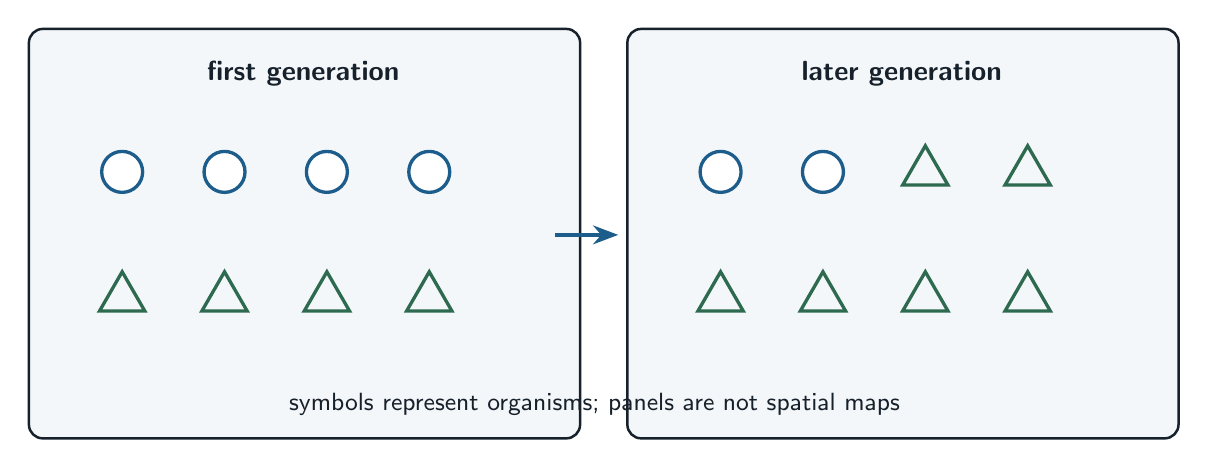
\begin{tikzpicture}[fc text, x=1cm, y=1cm]
  \node[fc panel, minimum width=70mm, minimum height=52mm, anchor=south west] at (0,0) {};
  \node[fc panel, minimum width=70mm, minimum height=52mm, anchor=south west] at (7.6,0) {};
  \node[fc label] at (3.5,4.65) {first generation};
  \node[fc label] at (11.1,4.65) {later generation};
  \foreach \x/\y in {1.2/3.4,2.5/3.4,3.8/3.4,5.1/3.4} {\draw[draw=fcblue, fill=white, line width=1.2pt] (\x,\y) circle (2.6mm);}
  \foreach \x/\y in {1.2/1.8,2.5/1.8,3.8/1.8,5.1/1.8} {\node[draw=fcgreen, regular polygon, regular polygon sides=3, minimum size=6.5mm, line width=1.2pt] at (\x,\y) {};}
  \foreach \x/\y in {8.8/3.4,10.1/3.4} {\draw[draw=fcblue, fill=white, line width=1.2pt] (\x,\y) circle (2.6mm);}
  \foreach \x/\y in {11.4/3.4,12.7/3.4,8.8/1.8,10.1/1.8,11.4/1.8,12.7/1.8} {\node[draw=fcgreen, regular polygon, regular polygon sides=3, minimum size=6.5mm, line width=1.2pt] at (\x,\y) {};}
  \draw[fc arrow] (6.7,2.6)--(7.5,2.6);
  \node[fc note] at (7.2,0.45) {symbols represent organisms; panels are not spatial maps};
\end{tikzpicture}
\end{document}
